\setcounter{tocdepth}{4}
\setcounter{secnumdepth}{4}
\newcounter{subsubparagraph}[subsubparagraph]
\section{Unity}

\includegraphics{images/unityLogo.png}
\newline
Unity ist eine Entwicklungsumgebung hauptsächlich gedacht für die Spieleentwicklung. Eigentümer des Produkts ist Unity Technologies, die ihren Sitz in San Francisco haben. 
Das Unternehmen ist seit 2004 in Betrieb und arbeitet ausschließlich an Unity und dessen Services. Die wichtigsten Services hierbei sind Unity Multiplayer, Remote Settings, der Unity Asset Store und Unity Collaborate. 

\subsection{Unity Multiplayer}
Unity Multiplayer soll es Entwicklern ermöglichen leicht und schnell, auf Mehrspieler basierende, Spiele zu entwickeln. Der Service bietet Support für die Synchronisierung von Objektpositionen zwischen den Geräten, Serverseitige Commands, die Cheating deutlich erschweren, eine Unterscheidung zwischen Client und Server im Code, sodass Entwickler auch für Einzelspieler gedachte Projekte leicht umbauen können, und vieles mehr. Der wohl größte Vorteil ist die Inkludierung eines Lobbysystems. Spieler können Lobbys erstellen und diese für andere Spieler freischalten, sodass diese der Gruppe beitreten können. Immer mehr Mehrspielerspiele, wie „Battlefield“, „Counterstrike“ oder „Destiny“, benutzen Matchmaking um Spieler, die in derselben Region spielen, in Lobbys zusammenzuschließen, um sie zu füllen. Die Spieleindustrie geht immer mehr in die Richtung, der Servicespiele. Der Grund ist, dass Spiele immer teurer werden und große Publisher nicht mehr mit den 60 Euro pro Spiel auskommen. Sie versuchen die Spiele weiter zu monetarisieren, indem sie Spielinhalte ohne zusätzliche Kosten erst spät oder gar nicht erreichbar machen. Je langlebiger die Spiele sind, desto eher ist die Wahrscheinlichkeit, dass Spieler bereit sind mehr dafür zu zahlen. Erreicht wird diese Langlebigkeit durch periodische Updates und nicht zu Letzt durch Mehrspielermodi. Spiele wie „The Division“, „Destiny“ oder „Anthem“ werden in vergleichbar schlechten Zustand veröffentlicht, mit einer großen Karte zum Erkunden und einem Mehrspielermodus. Während der nächsten Jahre werden Bugs behoben und Inhalte hinzugefügt um Spieler zurück zu bringen. Dieser Trend ist in der jetzigen Form zwar nicht wünschenswert, es ist jedoch trotzdem wichtig, dass Entwickler die Möglichkeit dazu haben. 

\subsection{Remote Settings}
Viele Mehrspielerspiele, wie „First-Person-Shooter“, MOBAs oder MMOs, benötigen regelmäßige Patches, um die Spielbalance zu verändern. Dieses Thema ist enorm komplex, da viele Räder ineinander greifen. „League of Legends“ ist seit über 10 Jahren, mit über 200 Millionen registrierten Nutzern, aktiv. Unabhängig davon wird alle 14 Tage ein Patch ausgerollt, der bestimmte Charaktere stärker und andere wieder schwächer macht. Diese Patches will der Service „Remote Settings“ ablösen, indem er Entwicklern die Möglichkeit gibt, bestimmte Werte mit der Cloud zu synchronisieren, sodass diese jederzeit über ein Webinterface, ohne zusätzliche Patches, geändert werden können. Patches sind somit nur mehr für Fehlerbehebungen und zusätzliche Inhalte nötig.

\subsection{Unity Asset Store}
Der Asset Store ist direkt in die Engine eingebaut und ist somit ein zentraler Aspekt von Unity. Er ist vor allem für Prototypen enorm wichtig und hilft Entwicklern schnell ihre Ideen zu testen und verbessern. Im Store können Nutzer Scripts, Modelle, Animationen, Tools und vieles mehr hochladen und auch herunterladen. Eine simple, aber effektive Review-Implementation ist vorhanden um hochwertige Assets zu präferieren. Inhalte sind für fast jedes Szenario und jede Idee vorhanden und deren Preise reichen von kostenlos bis zu mehr als 100 Euro. Es sind viele Modellpakete vorhanden, die oft gratis sind und für die Prototypenphase, als Platzhalter, verwendet werden. Viele Entwickler laden auch selbst entwickelte Tools, für die Kameraführung oder die Terraingestaltung, hoch. 2017 sparten Entwickler über 1 Milliarde Dollar durch die Benutzung von Assets aus dem Store.
Der Store ist aber auch zum Teil Schuld an der schlechten Reputation, die Unity, seit einiger Zeit, plagt. Unzählige Spiele werden täglich in die mobilen App Stores hochgeladen, die nur aus Asset Store Inhalten bestehen, um billige Kopien bekannter Spiele zu machen. Auch ein Grund ist, die Verwendung der Marke Unity selbst. Unity bietet eine Gratisversion, dessen größte Unterscheidung die Inkludierung des Unity Logos, am Start des Spiels, ist. Bei Bezahlversionen hat man die Wahl und da die Erscheinung des Logos meist für billige Spiele steht, entschließen sich die meisten dagegen. Die Zeit des Hochfahrens wird bei Spielen meist für die zur Schau Stellung der Technologien verwendet und die Gameengines in Verwendung entwerfen oft angepasste Logos für wichtige Spieleveröffentlichungen. Unity ist die meist verwendetste Engine am Markt und auch die erste Wahl für viele Indie Entwickler. Spiele, wie „Ori and the Blind“, „Cuphead“, „Superhot“, „Hollow Knight“, „Subnautica“ oder „Overcooked“, sind eine der größten Indie Erfolgsgeschichten in den letzten Jahren aber auch Smartphone Klassiker, wie „Angry Birds“, „Temple Run“, „Crossy Road“ oder „Pokemon Go“ sind mit Unity entwickelt worden. Jedoch erscheint das Unity Logo kaum bei Spielstart, weswegen man diese Spiele nicht sofort damit in Verbindung bringt.

\subsection{Unity Collaborate}
Unity Collaborate ist Unitys in die Engine eingebaute Git Alternative, die ein einfaches Zusammenarbeiten ermöglichen soll. Es gibt gewisse Einschränkungen, die unter gewissen Bedingungen KO-Kriterien sein können. Für Teams bis vier Personen ist der Dienst zwar gratis, werden Accounts jedoch auch mehreren Geräten genutzt, kann es zu Fehlern kommen, die behoben werden können, sofern man sich für eine der Bezahloptionen entscheidet. Unity Collaborate ist ein simples Tool, jedoch ist das neben der größten Stärke auch eine nicht zu vernachlässigende Schwäche. Ohne Erweiterungen kann der Dienst keine Dateiinhalte lesen und so Dateien zusammenfügen, wie es Git zum Beispiel kann. Es kann nur Unterscheiden in geändert oder eben nicht. Je nach Workflow kann das zum Problem werden. Ist eine strikte Arbeitsteilung vorhanden, so reicht diese Implementierung aus und macht den Dienst, so zur idealen Wahl. Arbeiten oft mehrere Leute an der selben Datei, so kann man Erweiterungen einbauen, die zusätzliche Funktionalität bieten können. Leider bietet Unity keine solchen Erweiterungen und man ist auf Dritte angewiesen.

\subsection{Unity Preispolitik}
Unity bietet hier drei Optionen, die sich abhängig von der Teamgröße, im Preis ändern können. Für Einsteiger und Solo Entwickler ist die Gratis Version von Unity ausreichend. Man ist in keiner Weise in den Plattformen, für die Spiele entwickelt werden können, eingeschränkt und auch der Großteil der Services ist gratis verfügbar. Support wird von Unity nicht bereit gestellt. Um diesen in eingeschränkter Form genießen zu können, wird die, 25 Dollar pro Monat kostende, Plus Version benötigt. Zusätzlicher Cloud Speicherplatz und Zugang zu einem Übungskurs sind zusätzliche Boni. Um sowohl einen „Dark Mode“, als auch ein T-Shirt zu bekommen, benötigt man die, 125 Dollar kostende, Pro Version, die alle Features, wie 20 Prozent Rabatt auf Premium Assets, mehr Cloud Speicherplatz, Zugang zu Entwicklerkonferenzen und vieles mehr freischaltet. Für größere Teams bietet Unity individuelle Lösungen. Selbst wenn man die zusätzlichen Features der Bezahlversionen nicht benötigt, ist man ab einem gewissen Umsatz dazu verplichtet.

\subsection{Plattformen}
Unity unterstützt seit vielen Jahren alle neuen Plattformen, selbst wenn diese selbst noch in Entwicklung sind. Neben den Standardplattformen, wie X-Box, Playstation, Nintendo Switch, Android, Ios, Windows, Linux und Mac werden auch Fernseherbetriebssysteme, wie Samsungs Tizen OS, Apples tvOS oder Googles Android TV unterstützt. Plattformen der Zukunft wie Microsoft Mixed Reality, Gear VR, Google Cardboard, AR-Core und viele mehr, die sich auf Augmented Reality oder Virtual Reality fokussieren, werden zahlreich unterstützt, weshalb Unity hier eine Marktdominanz zeigt. Spiele werden meist für mehrere Plattformen veröffentlicht und ein Vorteil, den Unity bietet, ist es, die selbe Codebasis für alle Plattformen zu verwenden. Ludimus hat sowohl einen Android, als auch einen Windows Client, dennoch können beide Plattformen mit dem selben Code funktionieren. Muss oder soll es jedoch Unterscheidungen zwischen Plattformen geben, so bietet Unity auch hier eine Lösung. Plattformspezifischer Code wird für alle nicht relevanten Plattformen, aus dem Code heraus geschnitten. Häufige Anwendungen hierfür sind Filesysteme und deren verschiedene Pfade. 

\subsection{Mobile Entwicklung}
Neben der Virtual und der Augmented Reality, ist Unitys Hauptverwendungszweck die mobile Entwicklung für Ios und Android. Der Vorteil der gleichen Codebasis ist hier enorm wichtig, da diese zwei Systeme sehr unterschiedliche Entwicklungsworkflows haben und es nicht effizient ist, für mehrere Plattformen einzeln zu entwickeln. Selbst große Publisher wie Square Enix, greifen bei ihrem „Tomb Raider“ Smartphone Ableger auf Unity zurück, da sie laut eigener Angabe schnell einen vorzeigbaren Prototypen bauen konnten. Auch Blizzard benutzte Unity zur Entwicklung von ihrem Kartenspiel „Hearthstone“, welches sowohl einen Android und Ios, als auch einen Windows Client, besitzt und auch sie erwähnen die schnelle Entwicklungszeit. Es sind Erfolgsgeschichten, wie diese weswegen Unity unter Entwicklern einen sehr guten Ruf genießt, auch wenn die Öffentlichkeit davon nichts mitbekommt. 

\subsection{Community}
Durch den großen Erfolg bildete sich schon zu Beginn eine riesige Community, die durch Tutorials und Livestreams von Unity selbst inspiriert wurde. Hunderte hochqualifizierte Entwickler teilen deren Wissen mit Anfängern und helfen ihnen auf ihrem Weg zum ersten Erfolg. Die Tutorials reichen von Programmierkursen, über die Modellierung, bis hin zur Integration anderer Dienste in Unity. Die Gemeinschaft ist groß genug, sodass jedes gewünschte Verhalten dokumentiert worden ist, oder jeder aufgetretene Fehler behoben worden ist.

\subsection{Integration}
Unity bietet Integrationen mit vielen Modellierungs-, Zeichen- und Audiotools. Die zwei am meisten vorkommenden Kombinationen sind wohl: Unity und Blender und Unity und Photoshop.
\subsubsection{Unity und Blender} \label{sec:unity-blender}
Blender ist eine gratis Open Source Modellierungssoftware, die in viele Formate exportieren kann und auch eine ähnliche Community, wie Unity, bietet. In vielen Tutorials werden Unity und Blender gemeinsam verwendet, da beide Programme zwar Einsteigerfreundlich sind, jedoch auch enormes Potenzial haben, sofern gebraucht. 
\subsubsection{Unity und Photoshop}
Für die 2D Spieleentwicklung sind Sprites, also Bilder, enorm wichtig. Viele Guides empfehlen hier meist Photoshop, den sowohl verschiedene Layer als auch Animationen werden perfekt unterstützt, um einen reibungslosen Workflow zu garantieren.

\section{Entwicklung mit Unity}
Die Entwicklung in Unity ist in viele kleine Bereiche aufgeteilt. Logik implementiert man jedoch immer in C-Sharp, sofern man keine explizite Lizenz für C++ erworben hat. Im Laufe des Jahres 2019, soll jedoch eine Visual Scripting Lösung getestet werden. Visual Scripting ist eine Drag and Drop Art der Programmierung. Ein Programm besteht hier aus Nodes. Diese Nodes haben bestimmte Funktionen, die miteinander verbunden werden können. Entwickler können eigene Nodes schreiben, um die Grundfunktionalität zu erweitern. Das bekannteste Beispiel dieser Entwicklungsmethode ist die Unreal Engine 4, die dieses Konzept schon seit Beginn nutzt. 
\subsection{Editor}
\begin{figure}
    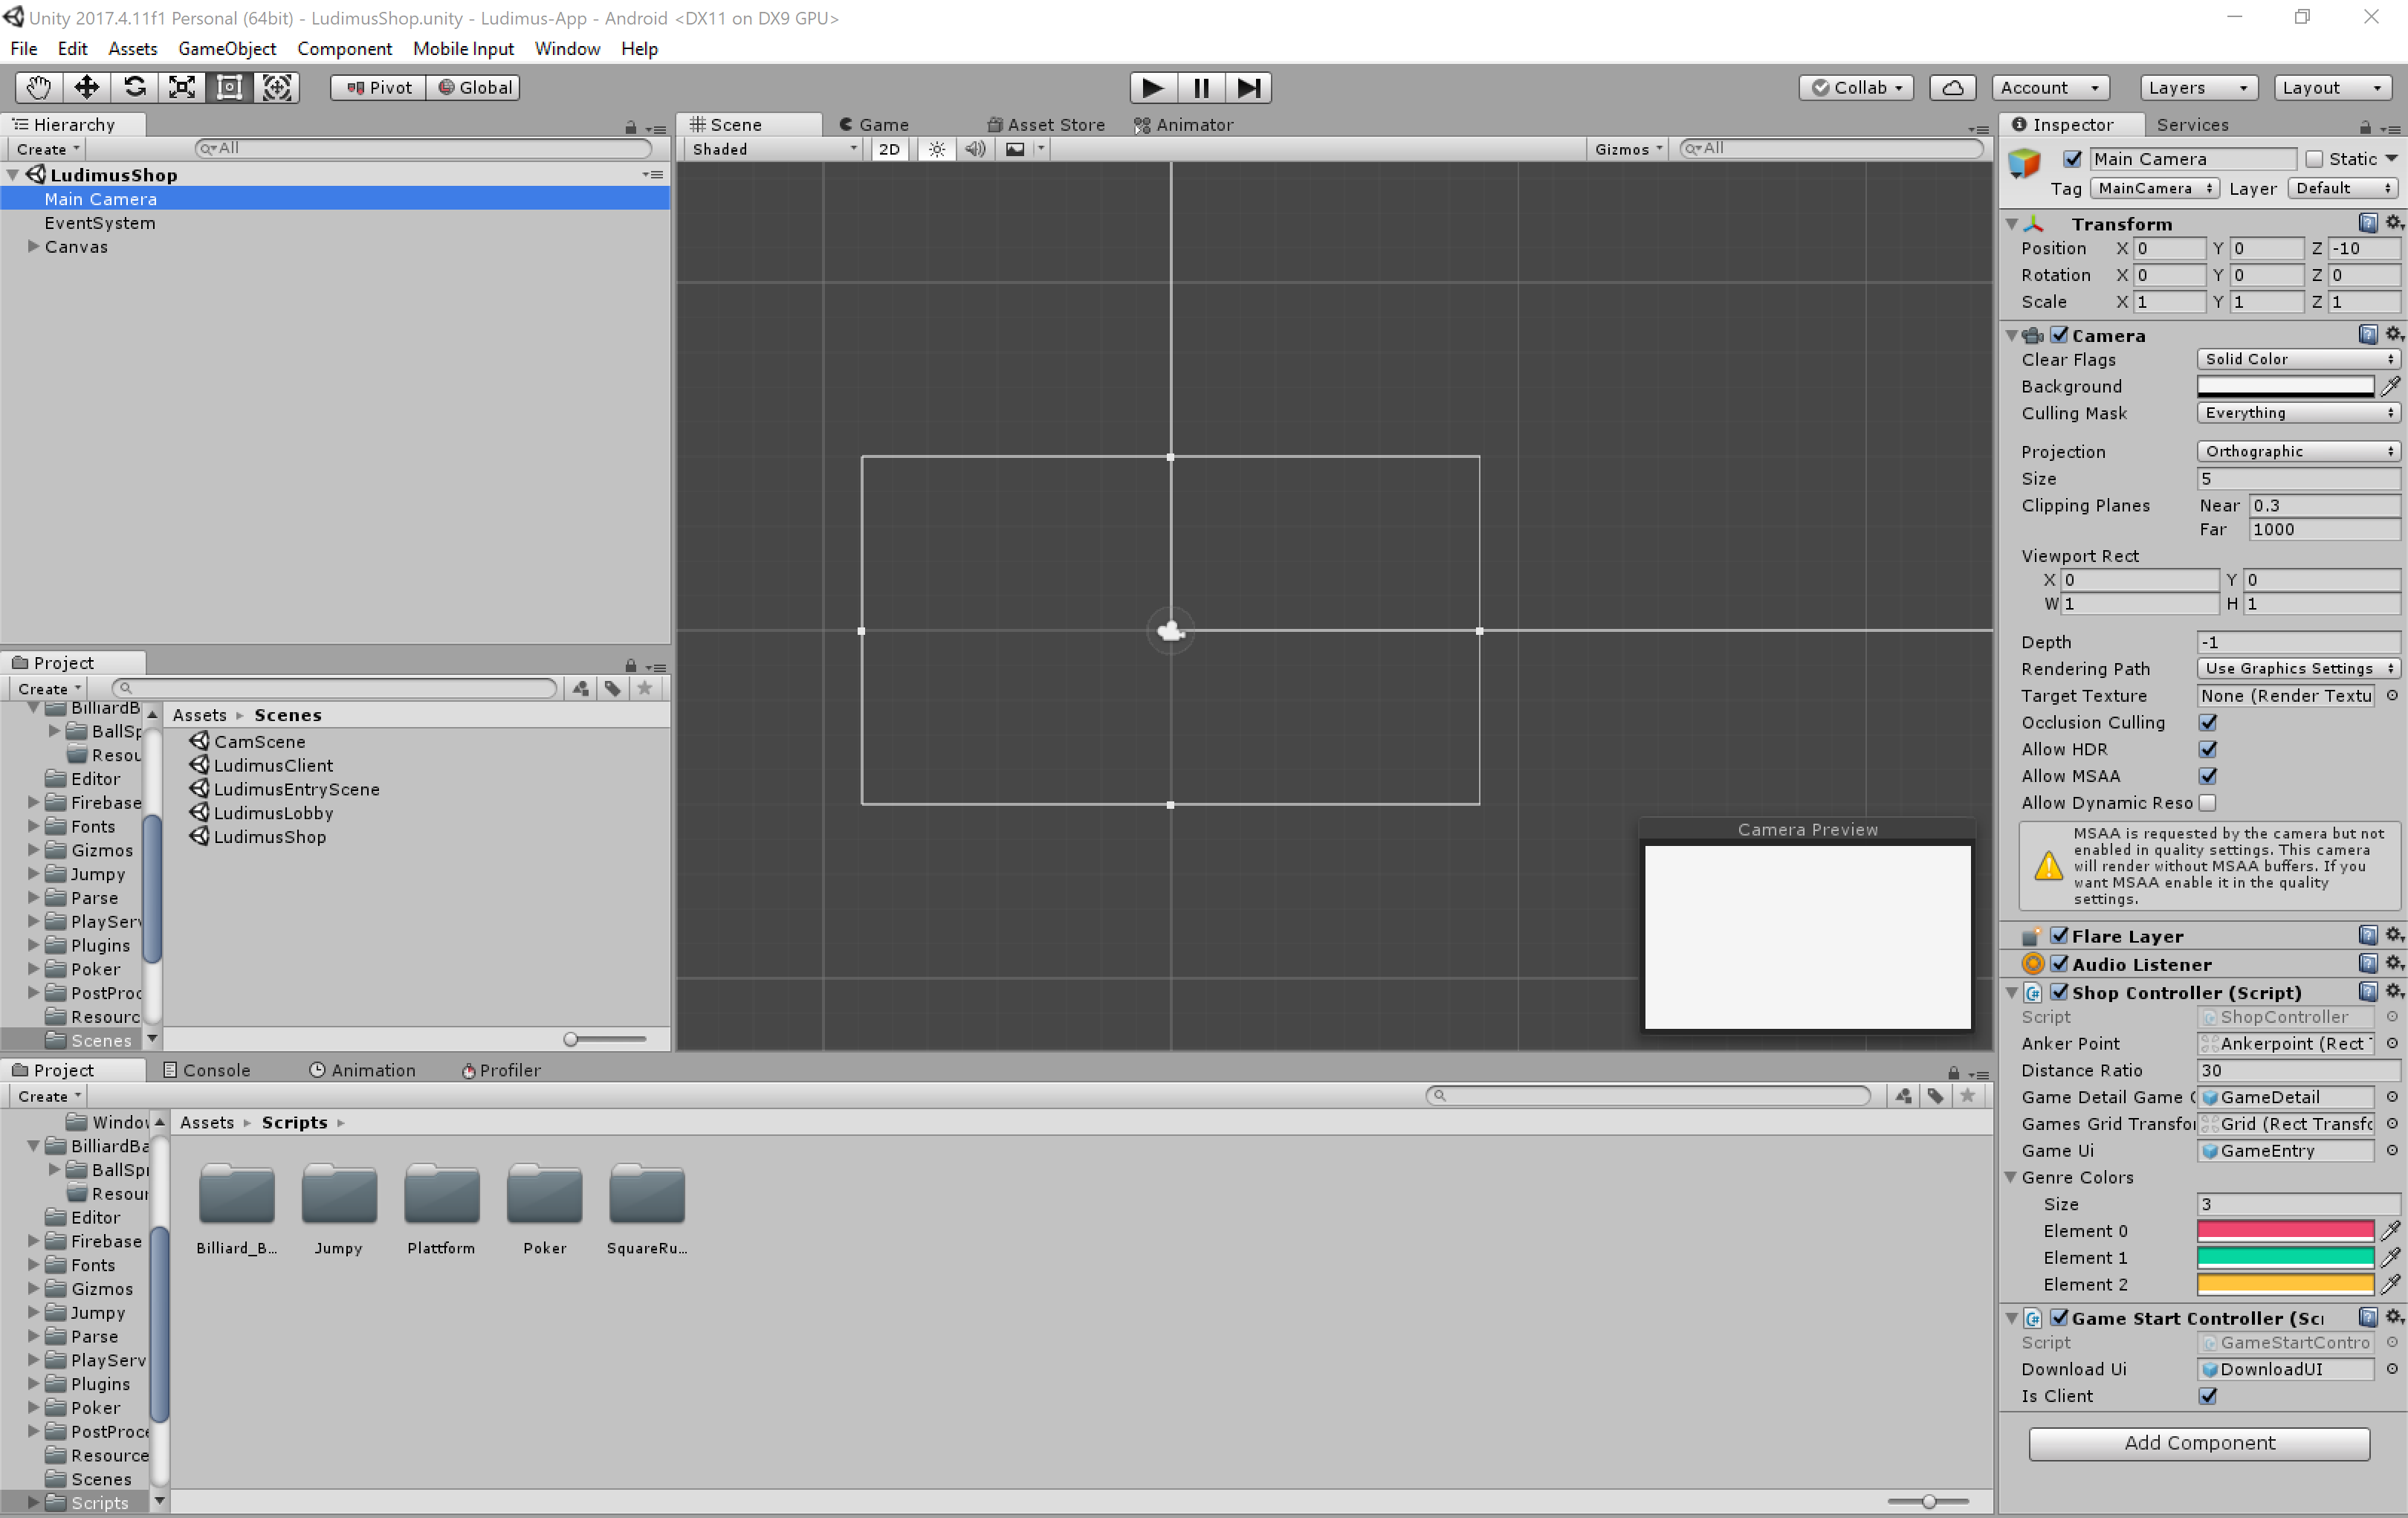
\includegraphics[scale=0.35]{images/unityEditor.png} 
    \caption{Unity Editor}
    \label{img:unity-editor}
\end{figure}

Der Editor ist in Tabs gegliedert, wie in Abbildung \ref{img:unity-editor} zu sehen, die beliebig angeordnet werden können. Wichtige Tabs sind:
\subsubsection{Hierarchy}
Hier werden alle Objekte, die in der aktuell ausgewählten Szene sind, angezeigt. Objekte können verschachtelt sein oder unabhängig voneinander herumverschoben werden. Die Details der ausgewählten Elemente werden im Inspector angezeigt.
\subsubsection{Scene}
Das Scene Fenster zeigt die Welt, die aktuell ausgewählte Szene, in der die Objekte existieren. Alle Objekte haben eine eindeutige Position, mit einer x, y und z Koordinate. Der Benutzer kann sich in diesem Dreidimensionalen Raum frei bewegen und Objekte anordnen, um seine Level zu gestalten. Da Unity sowohl 2D als auch 3D Entwicklung unterstützt, kann man die Perspektive einstellen.
\subsubsection{Project}
Der Project Tab die In Engine Version des Fileexplorers. Er verfügt über eine schnellere Suchfunktion und ein Favoritensystem. Hier ausgewählte Objekte können sowohl in die aktuelle Szene hineingezogen werden oder die Details, im Inspector, angesehen werden.
\subsubsection{Console}
Die Konsole zeigt alle Konsolen Einträge auf, gruppiert nach Art, sprich „log“, „warning“ oder „error“. Wählt man einen Eintrag aus, so sieht man dessen Details und kann auch zur Zeile im Code springen, der diesen ausgelöst hat. Die Standard Lösung von Unity verfügt über keine Suchfunktion, jedoch gibt es Tools im Asset Store, die diese Lücke füllen.
\subsubsection{Animation}
Soll sein Spiel über bewegliche Inhalte verfügen, so sind Animationen oft eine gute Lösung. Unity verwendet hier das Keyframe Prinzip, bei dem alle Eigenschaften zu zwei bestimmten Zeitpunkten, Keyframes, gespeichert werden, und anschließend alle Änderungen über die Zeit verteilt durch geführt werden. Unity unterstützt diese Art der Animation für 3D-Modelle, Sprites und UI-Elemente. 3D-Modelle und Sprites können mit einem Skelett versehen werden, dass bewegt werden kann um auch das Modell selbst zu bewegen.
\subsubsection{Game}
Ist es Zeit das Programm zu testen, so kann man es mithilfe des großen Spielen-Knopf starten. Unity wechselt danach automatisch in den Game Tab. Hier sieht man seine Szene durch eine Kamera, genauso wie sie Spieler später sehen würden. Dieser Modus ist für schnelle Testläufe ideal. Es gibt jedoch unterschiede zwischen dieser spielbaren Version und einer gebauten App, weshalb es ratsam ist, beide Versionen zu überprüfen.
\subsection{Komponenten}
Objekte in Unity bestehen aus Komponenten. Diese geben ihnen ihre Funktionalität und bieten gleichzeitig Flexibilität. Alle vom Entwickler generierten Scripts erben automatisch von der Basisklasse MonoBehaviour, wodurch sie als Komponenten verwendet werden können. Als Basis bietet Unity jedoch schon eine Reihe an Komponenten an, um Beispielsweise ein Objekt auf Gravitation reagieren zu lassen. Diese bereitgestellten Komponenten sind eingeteilt in: Mesh, Effects, Physics, Navigation, Audio, Video, Rendering, UI, AR und vielen mehr.
\subsubsection{Mesh}
Diese Gruppe besteht aus 3 verschiedenen und essentiellen Komponenten, für die 3D Entwicklung. Der Mesh Filter gibt an welches Modell dieses Objekt darstellen soll. Der Mesh Renderer hingegen beschreibt, welche Materialien das Objekt bekommt oder ob es Schatten erhalten oder werfen soll. Um 3D Text in der Szene anzuzeigen, benötigt man den Text Mesh Komponenten.
\subsubsection{Effects}
Egal ob Lagerfeuer, kleine Luftsteifen, um Bewegung deutlicher zu machen, oder Lens Flare Effekte, wenn der Spieler in die Sonne sieht, Effekte sind in Spielen häufig verwendet und Unity bietet hier eine gute Basis um seine eigenen Effekte zu erzeugen.
\subsubsection{Physics}
Dieser Punkt ist unterteilt in 2D und 3D Physics, um für Klarheit zu sorgen.
\paragraph{2D Physics}
Um die vorher erwähnte Gravitation für dieses Objekt zu aktivieren, benötigt man einen Rigidbody, hier konkret Rigidbody2D. Unity bietet eine globale Vektor Variable für die Gravitation, mit einer x und einer y Richtung. Im Rigidbody kann man die Stärke des Effekts auf dieses eine Objekt verändern. Die Werte für Masse, Trägheit und verschiedene Physics Materialien können eingetragen werden. Letztere bestimmen, wie stark das Objekt von Reibung beeinflusst wird und wie federnd es ist. Objekte können auch in ihrer Bewegung oder Rotation für verschiedene Achsen eingeschränkt werden.
Zusätzlich zum Rigidbody findet man hier alle Arten von Collidern, die Unity für 2D zu bieten hat. Diese Collider beschreiben die Zone, in der Kollisionen registriert werden. Collider können miteinander verknüpft werden, um die Objekte perfekt einzuhüllen. Box-, Circle-, Edge- und Polygon-Collider sind die am häufigsten verwendeten. Während Box- und Circle-Collider nur geometrische Formen beschreiben und lediglich in deren Größe geändert werden können, bieten sowohl Edge-, als auch Polygon-Collider Möglichkeiten, die für 3D nicht denkbar sind. Edge-Collider werden oft für Plattformen verwendet, da sie nur eine Linie darstellen, die an verschiedenen Punkten abgebogen werden kann. Das selbe Prinzip verfolgt der Polygon-Collider, nur verbindet er Start- und Endpunkt miteinander. Hinzukommt eine automatische Erkennung, der Form, bei Sprites. 
Als dritte Gruppe dieser Kategorie gelten die Joints. In verschiedenen Ausführung regeln sie das Verhalten zwischen zwei Objekten. Räder, Dämpfungen, Seile und mehr können so realisiert werden.
Zu guter Letzt gibt es noch Effectors. Diese regeln die Bewegungen, wenn zwei Objekte miteinander kollidieren. So können „One-Way“ Plattformen oder Förderbänder geschaffen werden.
\paragraph{3D Physics}
Die Rigidbody Implementierung für den dreidimensionalen Raum stellt eine abgespeckte Version, im Vergleich zur 2D, dar. Hier kann die Gravitation nur ein- oder ausgeschaltet werden und keine Physics Materialien zugeteilt werden.
Bei den Collidern finden sich Implementierungen der Standard Formen, wie Würfel oder Kreis ,wieder, hinzugekommen sind jedoch der Mesh Collider, der eine ähnliche Funktionsweise, wie der Polygon-Collider, darstellt und der Wheel Collider, der detaillierte Entscheidungsmöglichkeiten bezüglich Reifendruck, Federung, Reibung, in verschiedene Richtungen, und vielen mehr, bietet. 
Auch Effectors werden hier wieder aufgelistet, jedoch ist sticht die Cloth Komponente hier heraus. Sie ermöglich es Kleidung zu simulieren, um zum Beispiel im Wind zu flattern.
\subsubsection{Navigation}
Navigation ist nur für 3d Projekte verwendbar und ermöglicht es Entwicklern für jeder Objekt einzustellen, ob es begehbar ist, um anschließend Gegnerobjekten, oder anderen Objekten, die Wegfindung benötigen, einen sogenannten Nav Mesh Agent zu geben. Dieser Agent enthält Werte für Höhe, die maximale Schräge, die er bezwingen kann, und die maximale Stufenhöhe. Der Entwickler muss nur noch ein Ziel übergeben und das Objekt kann sich selbstständig dorthin bewegen.
\subsubsection{Audio}
Hier können Entwickler Objekte mit Fähigkeiten für das Zuhören oder das Sprechen ausstatten. Bestimmte Audiofilter für Echoeffekte können auch erstellt werden.
\subsubsection{Video}
Als einziges Element in dieser Gruppe, ist der Video Player das Werkzeug zum Präsentieren von vorher gerenderten Zwischenszenen.
\subsubsection{Rendering}
In jedem Spiel wird eine virtuelle Kamera verwendet, durch deren Linse gespielt wird. Diese Kamera Komponente ist unter dem Begriff Rendering, mit einer Skybox-, einer Licht- und der Sprite Renderer Komponente zu finden.
\paragraph{Camera}
Hier können wichtige Einstellung bezüglich der Darstellung getroffen werden. Von oben beginnend, kann der Entwickler gleich den Hintergrund festlegen. Standardmäßig ist er blau. Neben Farben können Entwickler jedoch auch Skyboxen auswählen. Mit der Option der Culling Mask, können bestimmte Schichten aktiviert oder deaktiviert werden. Die Projektion beschreibt die Art, wie mit entfernten Objekten umgegangen werden soll. Während Perspective Objekte, die in der Ferne liegen kleiner darstellt und so für 3D Spiel ideal ist, behält Orthograpfic die Originalgröße der Objekte unabhängig von deren Entfernung zu Kamera bei und eignet sich somit für 2D Spiele. Abhängig davon kann der Entwickler das Field of View oder die Kameragröße einstellen. Um zu verändern wie nah oder fern Objekte von der Kamera entfernt sein dürfen um gesehen zu werden, dient die Clipping Planes Option. Die restlichen Optionen sind für verschiedene Rendering Arten oder ob das gerenderte Bild gespeichert werden soll, um eine Karte zu erzeugen.
\paragraph{Skybox}
Die Skybox Komponente wird verwendet, um einen Himmel zu simulieren. Dazu benötigt man ein Skybox Material, welches dann hier verwendet werden kann.
\paragraph{Light}
Die Licht Komponente wird verwendet um Sonnenlicht, Licht von Lampen, Lagerfeuer und mehr zu simulieren. Dieses breite Aufgabengebiet wird mittels Untertypen realisiert.
\subparagraph{PointLight}
Punktlichter erleuchten einen bestimmten Bereich von einem Punkt aus in alle Richtungen. Lagerfeuer oder Lampen sind hier die Einsatzzwecke.
\subparagraph{Arealight}
Licht wird von einem bestimmten Punkt in einer Kegelform, in eine Richtung, versendet. Diese Methode ist für Scheinwerfer oder Spezielle Straßenlaternen sehr nützlich.
\subparagraph{Directionlight}
Um die Sonne zu simulieren, werden direktionale Lichter verwendet. Diese werfen Licht von überall in eine bestimmte Richtung, weshalb die Position keine Rolle spielt. 
\paragraph{Sprite Renderer}
Diese Komponente ermöglicht es Sprites in der Welt anzuzeigen. Das ausgewählte Sprite kann in der Farbe im Editor geändert werden, weshalb Sprites oft in Grautönen eingelesen werden, um sie in der Engine anzupassen, durch die Änderung des Order Layer vor oder hinter anderen Sprites angezeigt werden oder durch Materialen bestimmte Effekte, wie Wasserreflexionen, erhalten.
\subsubsection{UI}
Alle Komponenten, die mit der Erstellung eines Userinterfaces zusammen hängen, sind hier untergebracht. Es sind Presets für Buttons, Dropdown Menüs, Eingabefelder und vieles mehr vorhanden. UI-Elemente werden wie normale Objekte im dreidimensionalen Raum gesehen, weshalb Elemente auch nicht mit Code, wie html oder css, erzeugt und verändert werden können. 
\subsubsection{AR}
Je nach Plattform ändert sich die Größe dieses Menüs. SDKs für Geräte ähnlich der HoloLens bieten hier Komponenten für Spatial Recognition und mehr. 
\subsection{Scripts}
Diese Komponenten bieten ein solider Grundkonstrukt. Um Funktionalität in ein Spiel zu bringen werden jedoch, eigens geschriebene, Scripts benötigt, die wie folgt aufgebaut sind.
Wie bereits erwähnt, erben diese Programmteile von der Basisklasse MonoBehaviour. Lässt man sich die Scripts in der Engine generieren, so erhält man ein File ähnlich dem in Abbildung \ref{img:unity-basescript}.
\begin{figure}
    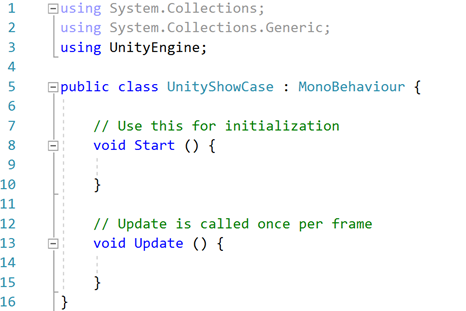
\includegraphics[scale=0.8]{images/unityScriptBase.png}
    \caption{Unity Basisscript}
    \label{img:unity-basescript}
\end{figure}
\subsubsection{Lifecycle Methoden}
Für Einsteiger sind die zwei generierten Methoden, Start und Update, kommentiert. Unity bietet verschiedene Lifecycle Methoden, die unterschiedliche Zwecke und Anwendungsbereiche haben, an.
\paragraph{Awake}
Die erste Methode, die für jedes Objekt aufgerufen wird ist Awake. Hier soll Code ausgeführt werden, der nur einmal ausgeführt werden darf.
\paragraph{OnEnable}
Objekte in Unity können jederzeit aktiviert oder deaktiviert werden. Werden Objekte aktiviert wird diese Methode aufgerufen. Diese Methode kann genutzt werden um andere Objekte auch zu aktivieren.
\paragraph{Start}
Start wird immer nach OnEnable aufgerufen und wird primär für die Verknüpfung zwischen Komponenten benutzt.
\paragraph{FixedUpdate}
Unity unterscheidet in zwei verschiedene Updatemethoden. FixedUpdate wird, wie der Name vermuten lässt, immer in selben Zeitintervallen aufgerufen, während Update immer dann verwendet wird, sobald ein neues Bild erschienen ist. FixedUpdate wird für Physikberechnungen und Eingabeüberprüfungen verwendet, die zwischengespeichert werden um in der Update Methode verwendet zu werden.
\paragraph{Update}
Hier wird die Logik des Spiels behandelt. Sollen Objekte bewegt werden, soll dies mit den vorher eingelesenen Werten hier geschehen. Haben bestimmte Aktivitäten eine Abklingzeit, bevor sie wieder verwendet werden können, so werden die Überprüfungen hier durchgeführt.
\paragraph{LateUpdate}
Wird für Kamerabewegungen genutzt und wird nach allen anderen Updates aufgerufen.
Anschließend wird das aktuelle Bild erzeugt und der Kreislauf beginnt bei FixedUpdate erneut.
\paragraph{OnDisable}
Wird ein Objekt während dieses Bildes deaktiviert, so wird diese Methode verwendet um zu reagieren. 
\paragraph{OnDestroy}
Wird dieses Objekt zerstört, zum Bespiel sobald der Spieler verloren hat, so dient diese Methode um den Score zu speichern oder ein bestimmtes UI aufzurufen.
\subsubsection{Kollisionen}
Kollisionen passieren, wenn zwei Collider desselben Typs, sprich 2D mit 2D und 3D mit 3D, miteinander kollidieren. Abhängig von deren Eigenschaften werden verschiedene Events aufgerufen.
\paragraph{OnCollisionEnter}
Kollidiert ein Collider mit einem anderen und beide haben die Standardeinstellungen ausgewählt, so wird diese Methode während dem Bild der Berührung aufgerufen.
\paragraph{OnCollisionEnter2D}
Ist das 2D Abbild der oben beschriebenen Methode.
\paragraph{OnCollisionStay/OnCollisionStay2D}
Solange zwei Collider miteinander kollidieren, wird diese Methode benutzt.
\paragraph{OnCollisionExit/OnCollisionExt2D}
Trennen sich die zwei Objekte nun wieder, kommt diese Methode zum Einsatz.
\subsubsection{Trigger}
Jeder Collider hat die Option ein Trigger zu sein oder nicht. Trigger registrieren zwar auf Kollisionen im Code, prallen jedoch nicht voneinander ab. Kollidiert ein Objekt, welches einen Collider mit einem aktiven Trigger hat, mit einem anderen Objekt, unabhängig von dessen Optionen, so werden folgende Events stattdessen ausgeführt.
\begin{description}
    \item OnTriggerEnter/OnTriggerEnter2D
    \item OnTriggerStay/OnTriggerStay2D
    \item OnTriggerExit/OnTriggerExit2D
\end{description}
\subsubsection{Objekte erzeugen}
Im Editor können Objekte mit Drag and Drop in die Szene hineingebracht werden. Will man jedoch zur Laufzeit Objekte erzeugen, so funktioniert dieser Ansatz nicht. Die Methode Instantiate erledigt dies, es gibt jedoch verschiedene Möglichkeiten diese zu benutzen.  Durch die letzten Parameter kann eingestellt werden, wo und als Kind welchen Elements das Objekt erzeugt wird. Im ersten Parameter muss man das Objekt selbst angeben, wobei der Entwickler hier 3 Optionen hat.
\paragraph{Resources}
Bestimmte Ordnernamen sind mit speziellen Funktionen belegt. Der StreamingAssets Ordner zum Bespiel ist für nicht zu kompilierende Inhalte bereitgestellt. Um Objekte einfach zu erzeugen, dient der Resources Ordner. Gespeicherte Objekte können aus diesem über ihren Name erzeugt werden mit der Zeile aus Abbildung \ref{img:unity-instantiate01}.
\begin{figure}
    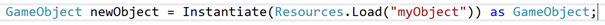
\includegraphics[scale=0.8]{images/unityInstantiate01.png}
    \caption{Objekt erzeugen über Resources}
    \label{img:unity-instantiate01}
\end{figure}
\begin{figure}
    
\includegraphics[scale=0.8]{images/unityInstantiate02.png}
    \caption{Objekt erzeugen durch Klonen eines Objektes}
    \label{img:unity-instantiate02}
\end{figure}
\paragraph{Klonen}
Um Objekte schnell klonen zu können, dient die Zeile aus \ref{img:unity-instantiate02}.

\paragraph{Referenzen}
Die selbe Syntax, jedoch einen anderen Verwendungszweck hat die Erstellung von Objekten mittels Referenzen. Ein Objekt kann als öffentliche Variable gespeichert werden, um später eine Instanz davon zu erstellen.
\subsubsection{Öffentliche Variable und Verlinkung zwischen Komponenten}
Unity bietet mehrere Möglichkeiten für die Erstellung von Referenzen zwischen Komponenten, wobei deren Einsatz sich deutlich unterscheidet.
Um auf Komponenten eines Objektes zugreifen zu können, benötigt man zuerst eine Referenz auf dieses Objekt selbst. Die Methode GetComponent() gibt anschließend den gewünschten Komponenten zurück. Referenzen auf Objekte kann man durch Filtern aller Objekte bekommen, zusehen in Abbildung \ref{img:unity-getallobjects}.
\begin{figure}
    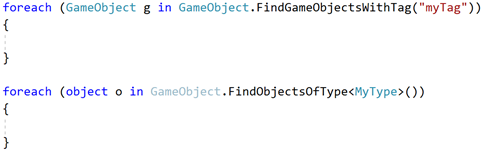
\includegraphics[scale=0.8]{images/unityGetAllObjects.png}
    \caption{Beschaffung aller Objekte mit einer bestimmten Eigenschaft}
    \label{img:unity-getallobjects}
\end{figure}
Objekte werden meist mit Tags versehen, weshalb die erste Methode öfter verwendet wird. Will man jedoch nur ein bestimmtes Objekt, so ist es nicht ratsam alle Objekte auf deren Namen zu überprüfen. Hier bietet Unity ein extrem brauchbares Features, welches bei öffentlichen Variablen Standard ist, jedoch mit der Annotation SerializeField auch für private Felder verwendet werden kann, siehe Abbildungen \ref{img:unity-serializefield} und \ref{img:unity-puplicfield}. Die Werte dieser Felder können über den Inspector gesetzt werden, wie in \ref{img:unity-inspectorsimple} und \ref{img:unity-inspectoradvanced} zu sehen.
\begin{figure}
    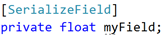
\includegraphics[scale=0.8]{images/unitySerializeField.png}
    \caption{Privates Feld mit SerializeField Annotation}
    \label{img:unity-serializefield}
\end{figure}
\begin{figure}
    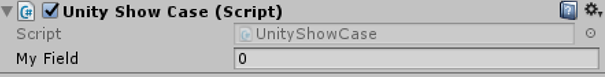
\includegraphics[scale=0.8]{images/unityInspectorSimple.png}
    \caption{Inspector Ansicht von Feldern}
    \label{img:unity-inspectorsimple}
\end{figure}

Erstellt man öffentliche Felder mit den Komponenten oder einem Objekt als Typ, wie in Abbildung \ref{img:unity-puplicfield}, so kann man diese im Inspector per Drag and Drop belegen, zu sehen in \ref{img:unity-inspectoradvanced}.
\begin{figure}
    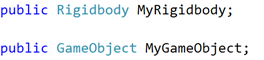
\includegraphics[scale=0.8]{images/unityPuplicField.png}
    \caption{Öffentliche Felder mit komplexen Datentypen}
    \label{img:unity-puplicfield}
\end{figure}
\begin{figure}
    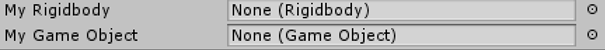
\includegraphics[scale=0.8]{images/unityInspectorAdvanced.png}
    \caption{Inspector Ansicht von mehreren komplexen Feldern}
    \label{img:unity-inspectoradvanced}
\end{figure}

Diese Methode wird verwendet, wenn Referenzen auf andere Objekte nötig sind. Den eigenen Rigidbody, sollte man jedoch nicht so referenzieren. Hier sollte eine private Variable angelegt werden, die mit GetComponent() in der Start Methode initialisiert wird, siehe Abbildung \ref{img:unity-getcomponent}.
\begin{figure}
    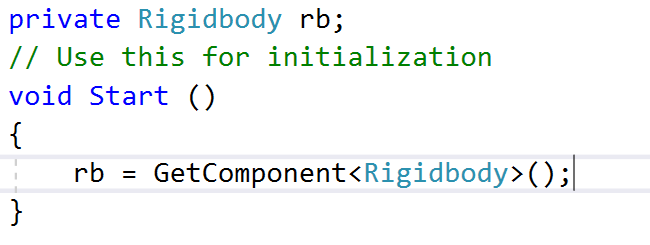
\includegraphics[scale=0.8]{images/unityGetComponent.png}
    \caption{Rigidbody des eigenen Objektes erhalten}
    \label{img:unity-getcomponent}
\end{figure}
\subsection{Alternativen}
Unity ist nicht die einzige Spieleengine und andere Optionen wie die Unreal Engine 4 oder Gamemaker Studio, wären valide Optionen gewesen. Unity bietet jedoch soliden Support für sowohl 2D als auch 3D, wodurch wir in keinster Weise eingeschränkt waren.  Den größten Vorteil der Unreal Engine, die unglaublich mächtige Rendering Pipeline, würde von unseren Spielen nie ausgereizt worden, weshalb wir uns für die Unity Game Engine entschieden, nicht zuletzt wegen unserer schon vorhandenen Erfahrung und der riesigen Community.